\documentclass{article}

\usepackage[utf8]{inputenc}
\usepackage{xcolor}
\usepackage{graphicx}
\usepackage{float}
\usepackage[margin=0.8in]{geometry}
\usepackage[italian]{babel}
\usepackage{hyperref}
\usepackage{minted}

\graphicspath{{./images/}}

\title{Relazione Progetto Algoritmi e Strutture Dati \\ A.A. 2021 - 2022}
\author{Antonutti Marco (142426)
        \and Candolo Vittorio Giorgio (141879)
        \and Pipan Martin (151699)}
\date{Dicembre 2022}
\begin{document}
\maketitle

\newpage
\renewcommand{\contentsname}{Indice}
\tableofcontents

\newpage

\section{Introduzione}
L'elaborato tratta l'attività di progettazione, implementazione e analisi di programmi che risolvono un problema computazionale di selezione.
\newline
\newline
Vengono presentate nella relazione le scelte implementative adottate e un'analisi della stima di complessità.

\newpage

\section{Algoritmi di selezione}

\subsection{Il problema della selezione}
Il problema della selezione è un problema algoritmico generale.
\newline
\newline
L'algoritmo che risolve il problema trova il k-esimo elemento più piccolo in un vettore.
\newline
Casi particolari possono considerarsi la ricerca del minimo, del mediano e del massimo.
\newline
\newline
Esistono soluzioni al problema in complessità $\Theta(n)$.
\newline
Per quanto riguarda la complessità spaziale esistono anche diverse soluzioni in place.
\newline
\newline
Il problema non è solo apparentemente correlato all'ordinamento, la selezione può essere sfruttata per ordinare un vettore (tramite applicazioni ripetute) e alcuni algoritmi di selezione sono derivati da algoritmi di ordinamento.

\subsection{Quick Select}
Questo algoritmo di selezione deriva da Quick Sort.
\newline
\newline
A differenza di quest'ultimo la ricorsione non avviene però sia alla sinistra che alla destra del pivot ma solo dalla parte che contiene il k-esimo elemento più piccolo (con conseguente riduzione di complessità).
\newline
\newline
Quick Select esegue un ordinamento parziale dell'input.
\newline
\newline
Le performance di questo algoritmo sono buone nel caso medio ma la complessità nel caso pessimo è $\Theta(n^2)$.
\newline
Ci sono quindi soluzioni preferibili dal punto di vista della complessità nel caso pessimo.
\newline
\newline
L'implementazione può anche essere in place e sono possibili varie ottimizzazioni di questo algoritmo quali la scelta random del pivot, diverse implementazioni di partition e, come vedremo, l'uso della mediana delle mediane come pivot.
\newline
\newline
Per quanto riguarda l'implementazione da noi scelta, essa è direttamente derivata da Quick Sort.
\newline
Per il partizionamento abbiamo preferito una versione di Lomuto Partition all'algoritmo di Hoare.
\newline
\newline
Non sono presenti ottimizzazioni di alcun genere.
\newline
Questa scelta implementativa è stata fatta per rimanere fedeli allo scopo del progetto e far emergere le differenze tra questo algoritmo e i successivi.
\newline
\newline
Da una breve sperimentazione di una variante facente uso dell'algoritmo di partizionamento di Hoare  e con scelta randomica del pivot, è emersa dall'analisi delle distribuzioni dei tempi di esecuzione una sensibile riduzione della deviazione standard rispetto alla versione da noi implementata.
\newline
\newline
Non essendo questo confronto oggetto del laboratorio non ci siamo dilungati in analisi più approfondite ma, anche al fine di testare il programma per la stima dei tempi di esecuzione, abbiamo prodotto due grafici (realizzati secondo modalità che saranno descritte in seguito) per riassumere il confronto empirico tra questa variante e la nostra implementazione.
\newline
\newline
In linea teorica l'algoritmo di Hoare è da preferire$^1$ rispetto al partizionamento Lomuto.
\newline
Per Quick Select vale che la scelta randomica del pivot quasi garantisce$^2$ la complessità lineare.
\newline
Riteniamo che le aspettative teoriche abbiano trovato riscontro empirico.
\newline
\newline
\newline
\newline
\newline
\newline
\href{https://cs.stackexchange.com/a/11550}{1. Quicksort Partitioning: Hoare vs. Lomuto}
\newline
\href{https://11011110.github.io/blog/2007/10/09/blum-style-analysis-of.html}{2. Blum-style analysis of Quickselect}

\newpage
\begin{center}
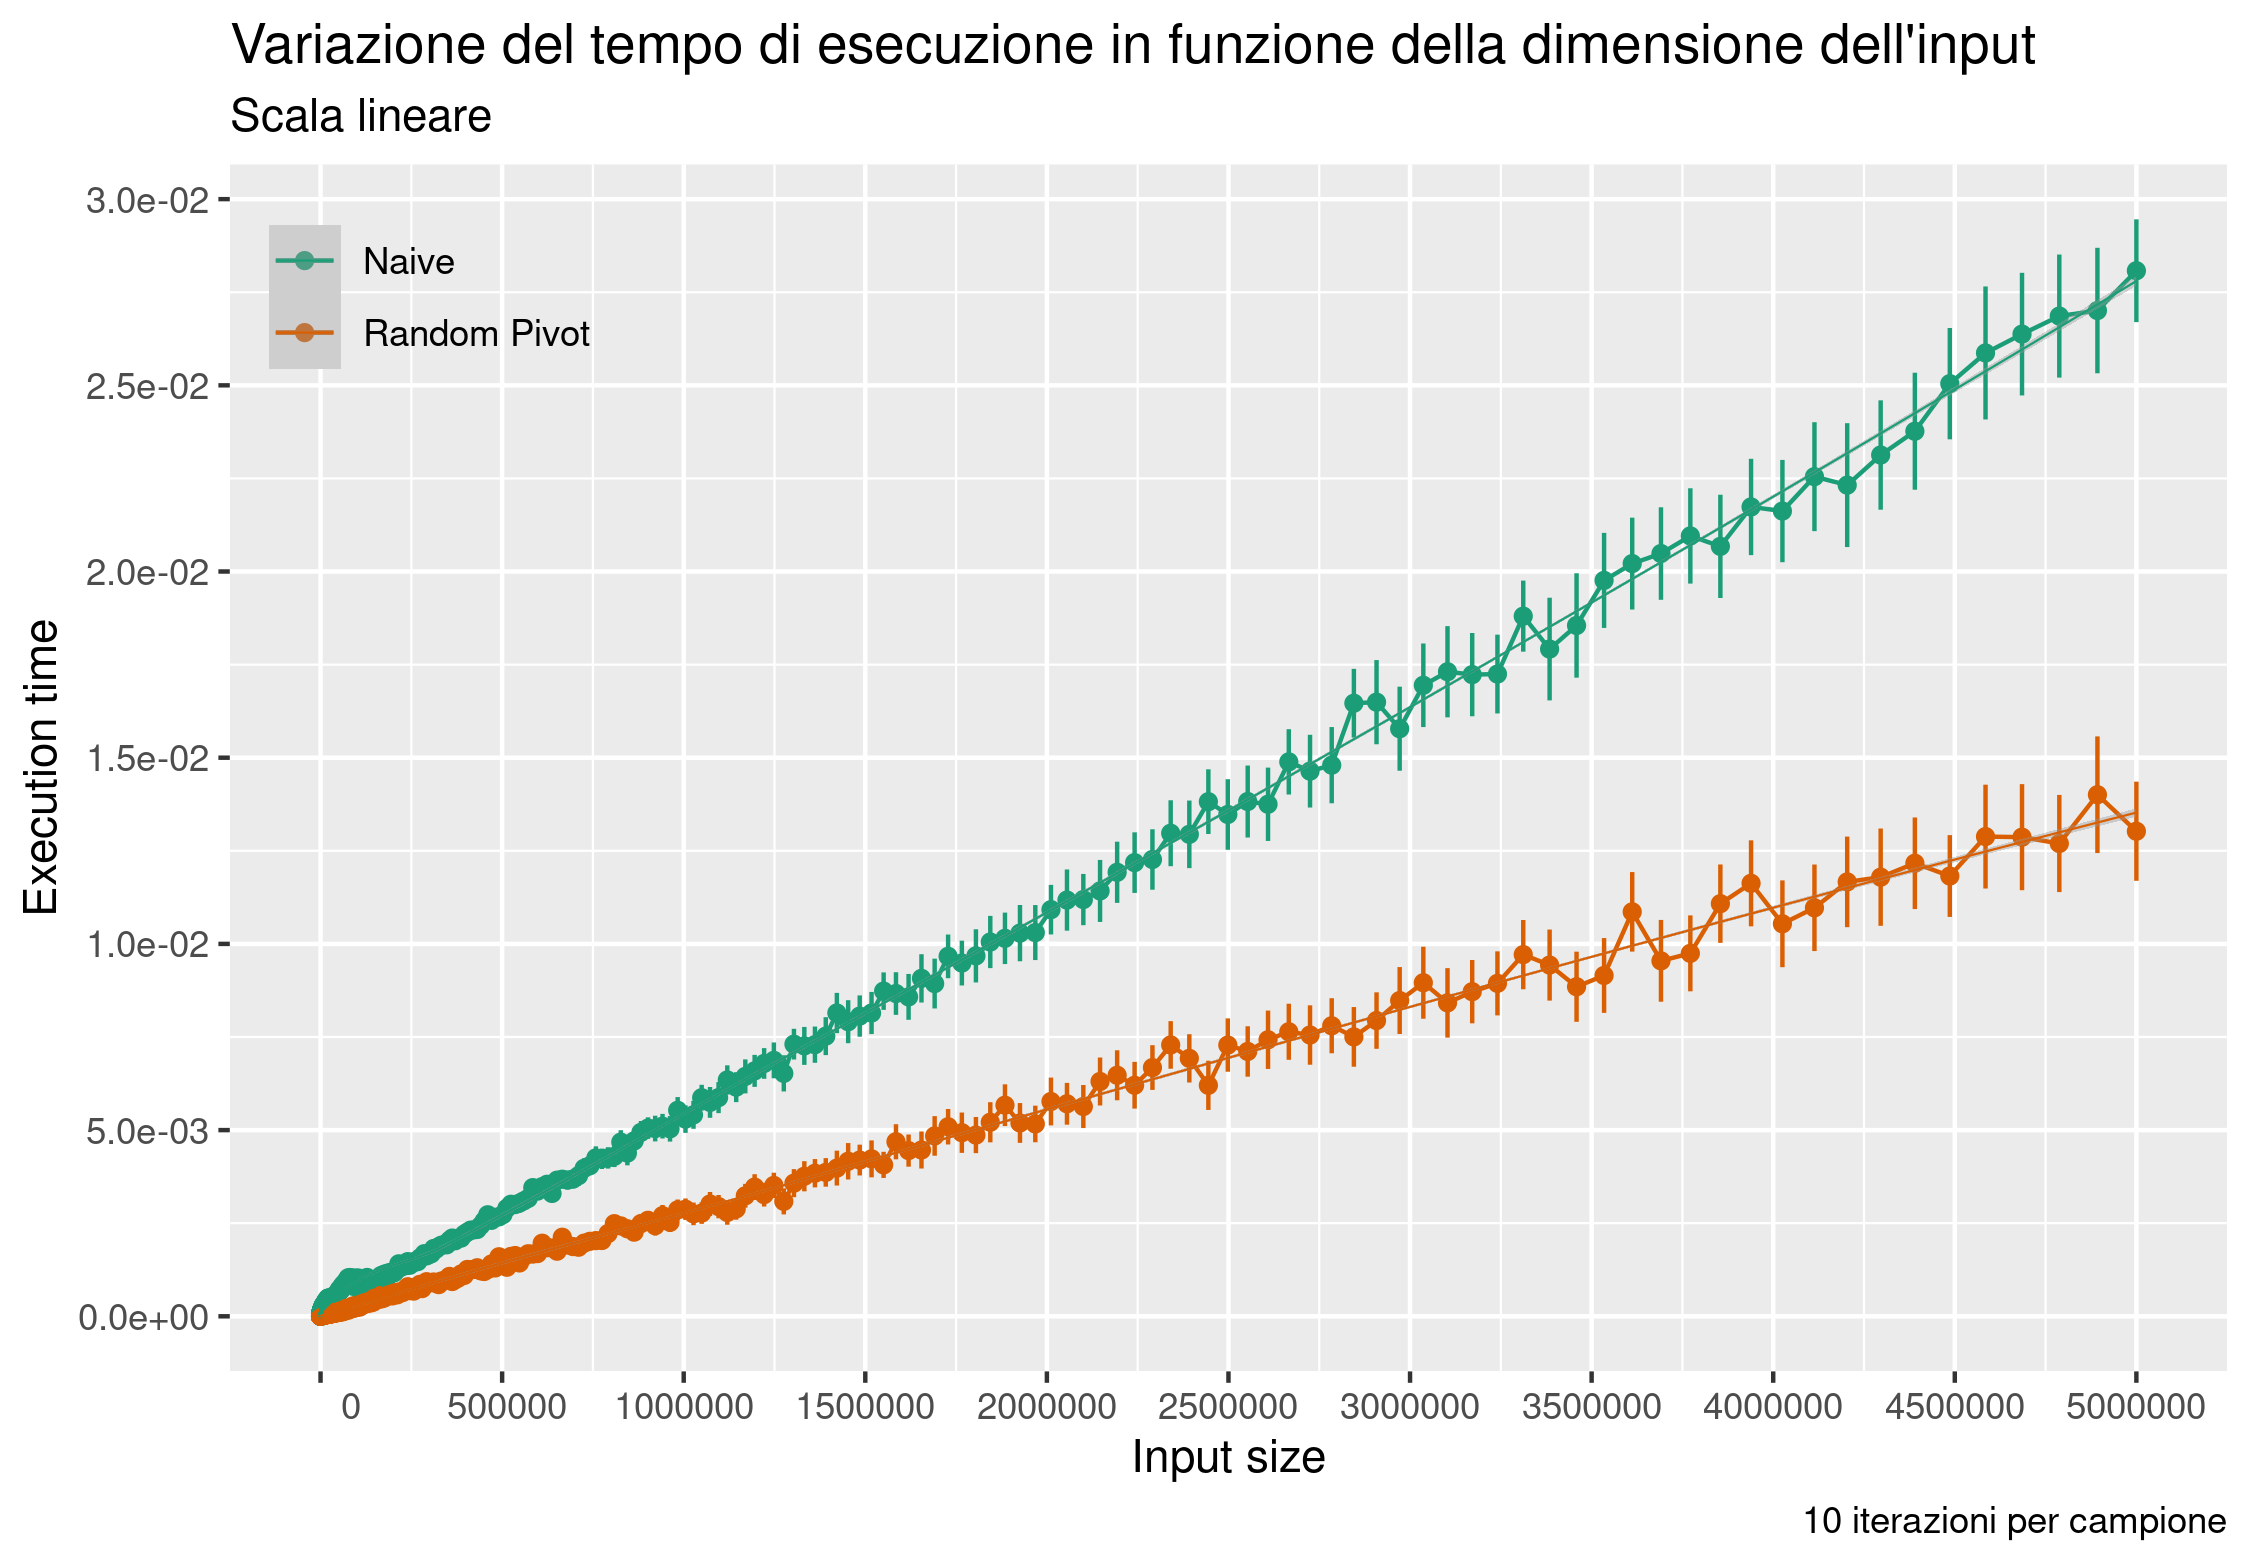
\includegraphics[width=0.97\textwidth]{qp_lin.png}
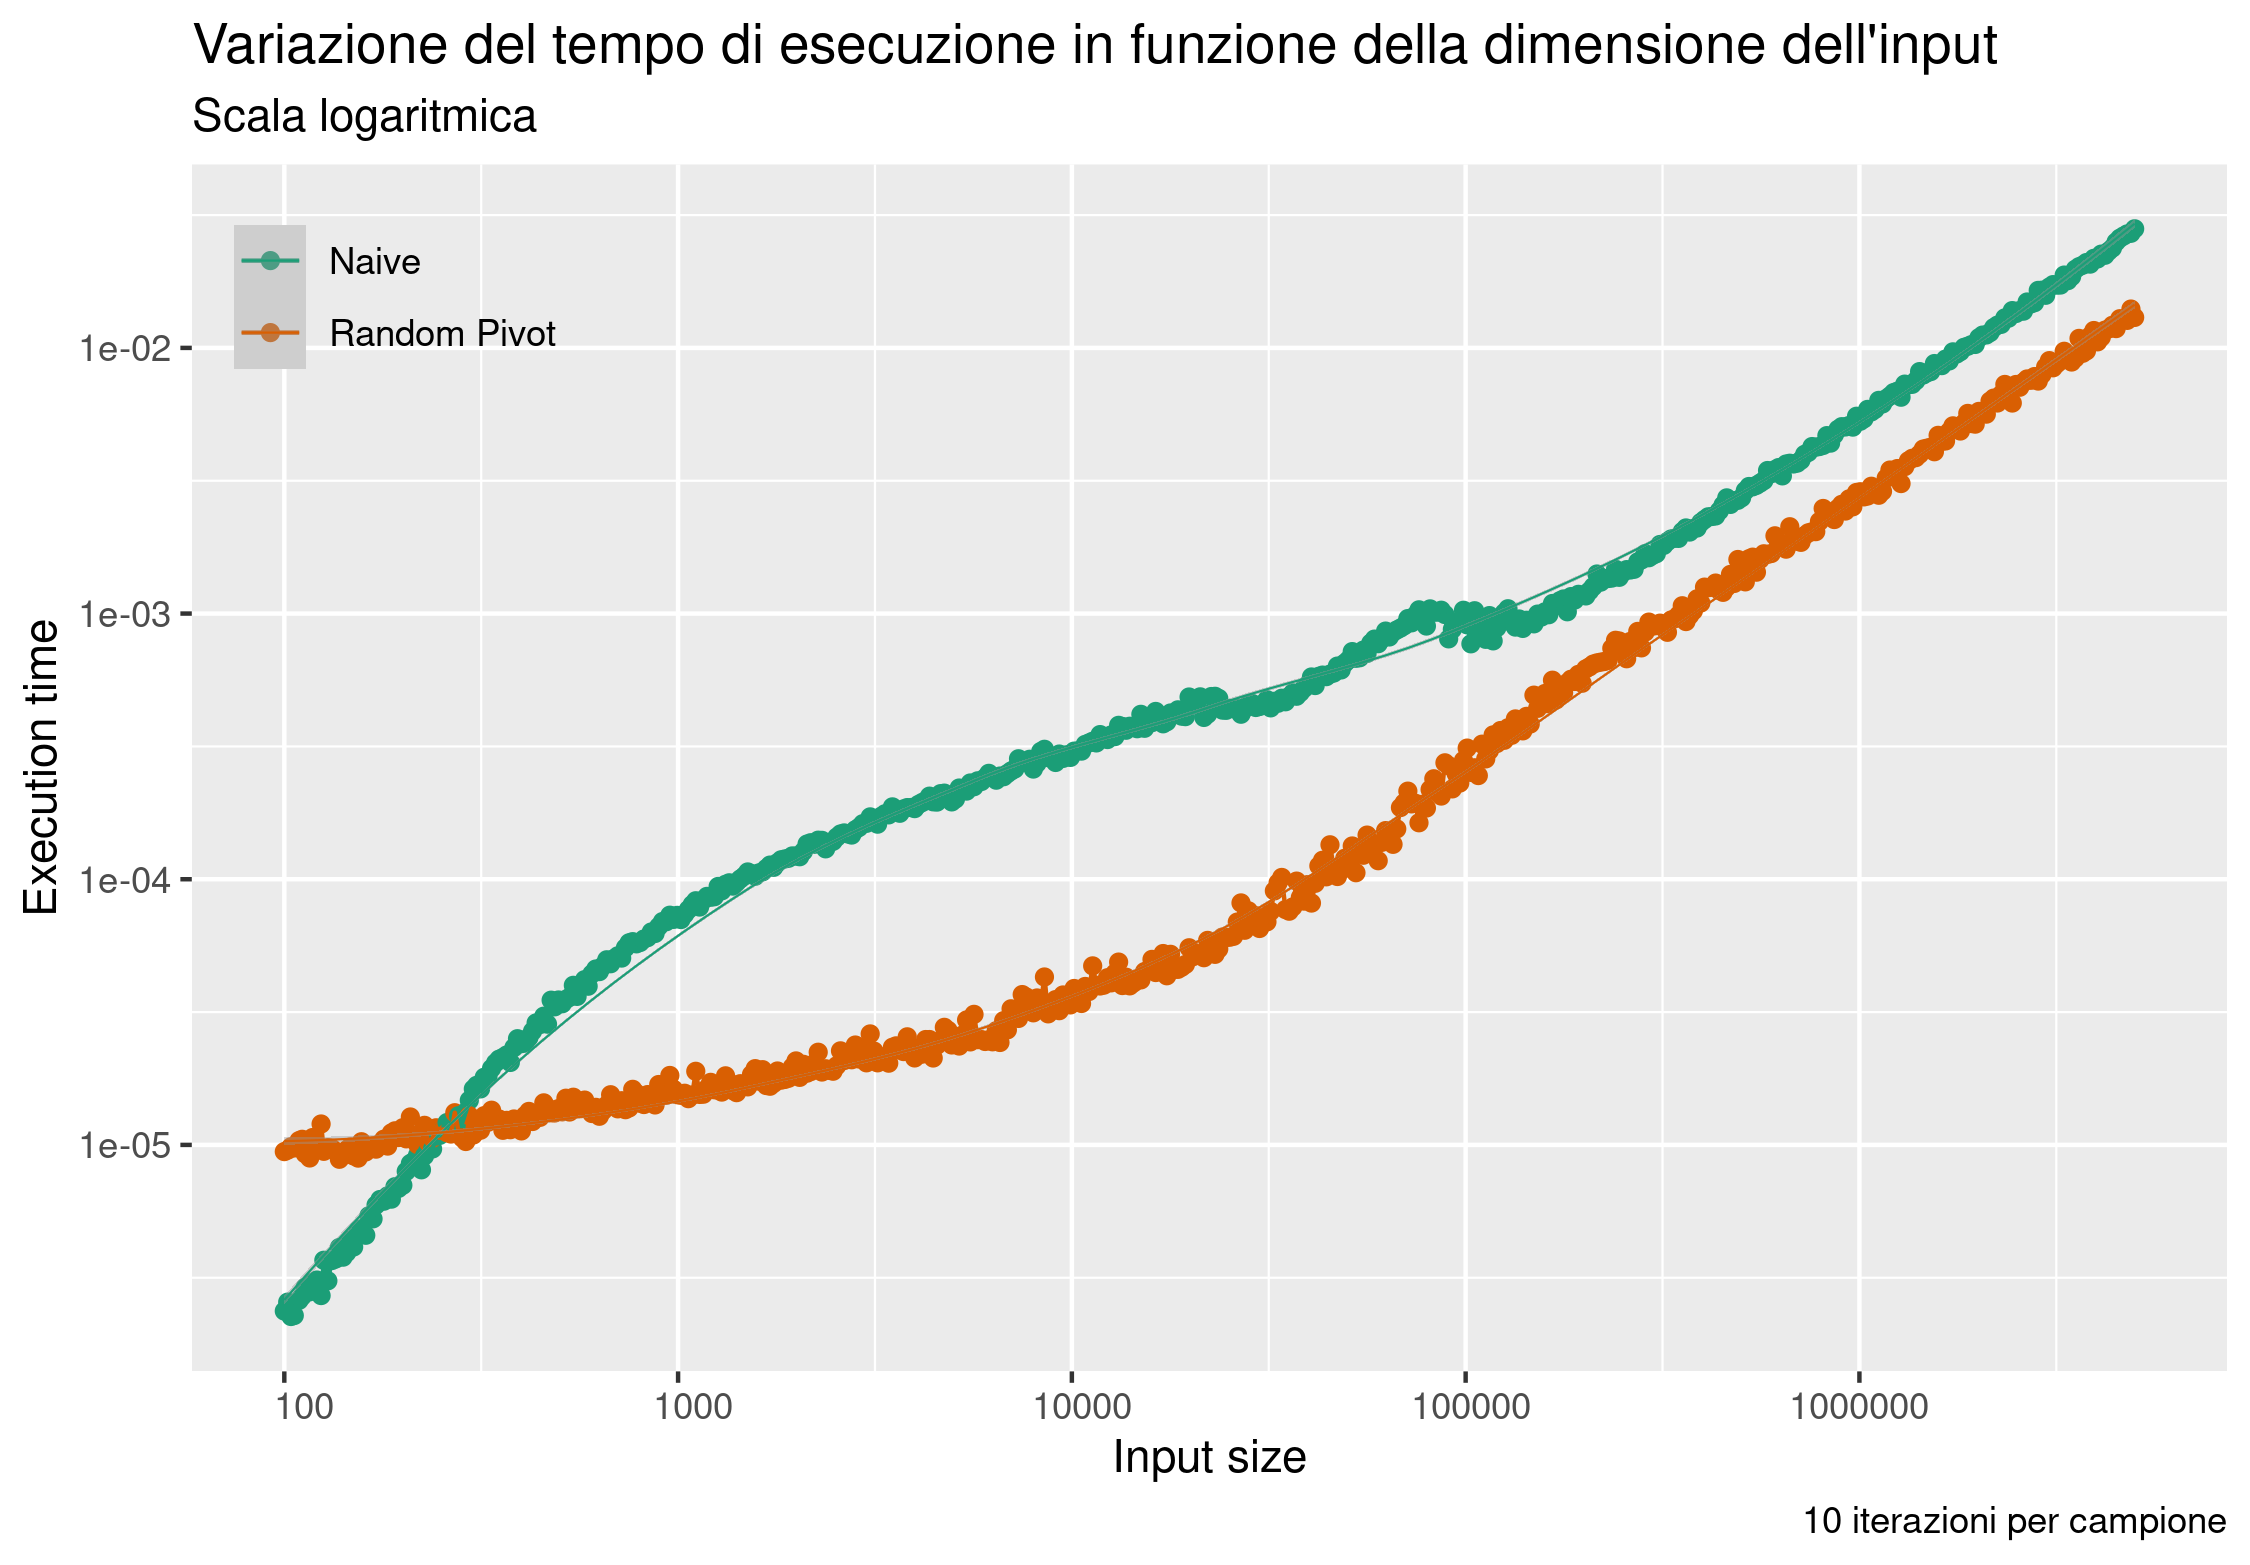
\includegraphics[width=0.97\textwidth]{qp_log.png}
\end{center}

\newpage

\subsection{Heap Select}
Heap Select è un algoritmo di selezione che sfrutta le heap, una struttura dati astratta.
\newline
\newline
La proprietà di heap che caratterizza la struttura si può così riassumere:
\newline
se A è un genitore di B, allora la chiave di A è ordinata rispetto alla chiave di B.
\newline
La relazione d'ordine deve essere uniforme per tutta la struttura, si distingue quindi tra min e max heap.
\begin{center}
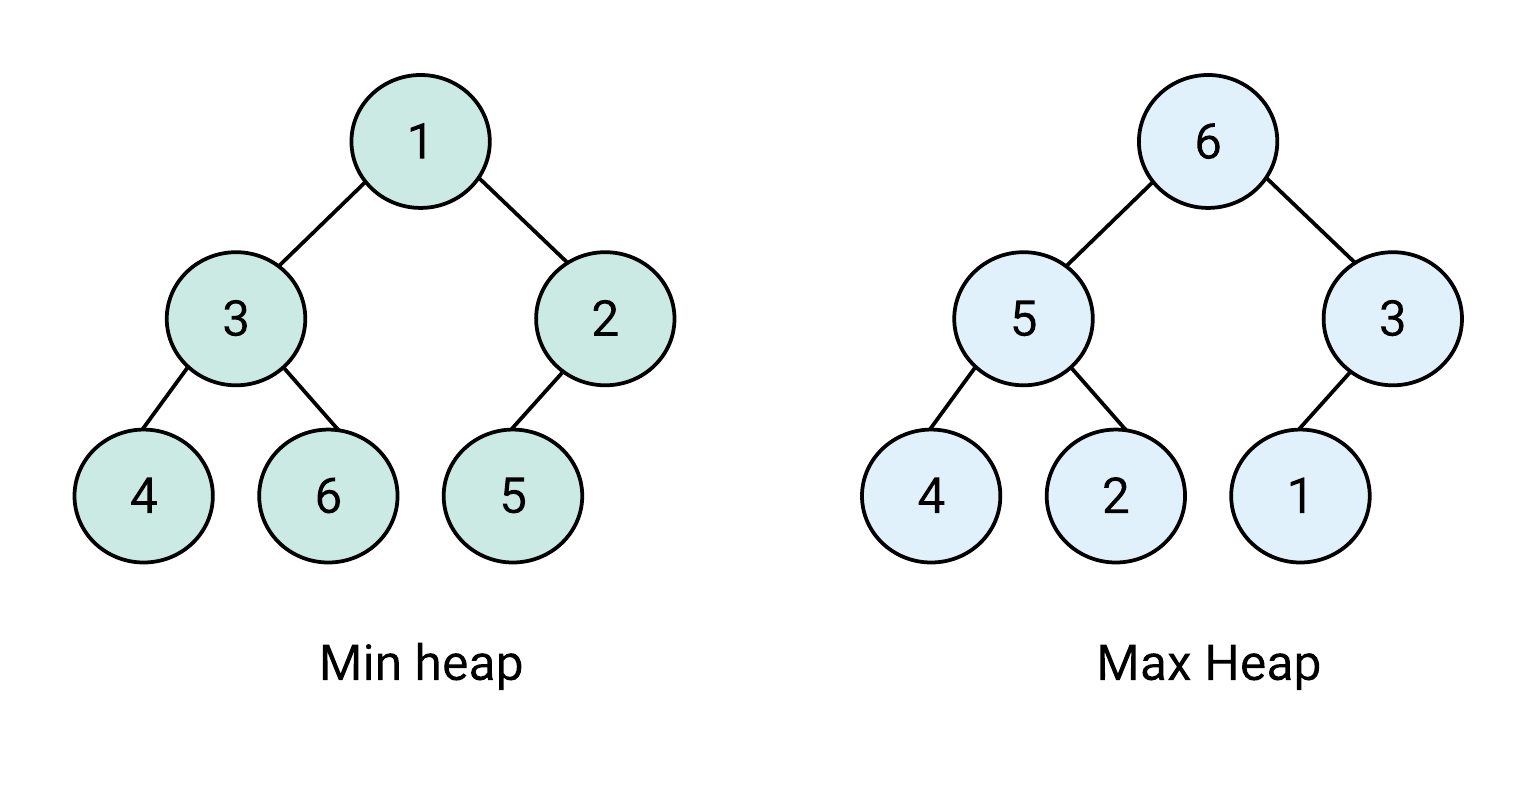
\includegraphics[width=0.5\textwidth]{heap.png}
\end{center}
Noti i metodi che caratterizzano la gestione di questa implementazione di coda con priorità è facile realizzare che per selezionare il k-esimo elemento più piccolo sia sufficiente estrarre k volte la radice di una min heap.
\newline
\newline
L'algoritmo di cui è richiesta l'implementazione è caratterizzato però da due heap.
\newline
La prima heap, costruita in tempo lineare, non viene mai modificata ma la sua radice viene copiata nella seconda.
\newline
\newline
La radice della seconda heap viene estratta e vengono inseriti in essa i suoi successori, dalla prima heap.
\newline
Questo iterativamente per k - 1 volte.
\newline
\newline
L' algoritmo ha una complessità $O(n + k log k)$ sia nel caso medio che in quello pessimo.
\newline
Ci si aspetta quindi che, per k sufficientemente piccoli, sia preferibile almeno rispetto al caso pessimo di Quick Select.
\newline
\newline
La versione da noi realizzata implementa la heap come un vettore di paia \textit{(chiave, posizione)}.
\newline
La posizione è necessaria per trovare i successori nell'algoritmo descritto in precedenza.
\newline
Si è scelto poi di implementare l'ottimizzazione relativa alla distinzione tra uso di min o max heap in base al valore di k (la struttura dati viene scelta in modo da garantire il numero minimo di iterazioni).
\newline
Dei tre algoritmi trattati è l'unico la cui implementazione ha previsto allocazione dinamica della memoria.
\newline
Per la costruzione in tempo lineare della prima heap si è sfruttato Heapify come noto.

\subsection{Median of Medians Select}
Questo algoritmo sfrutta Median of Medians per selezionare la mediana delle mediane che viene poi utilizzata come pivot ottimale in una procedura del tutto simile a quella vista con Quick Select.
\newline
\newline
Median of Medians Select è largamente impiegato in ragione del fatto che garantisce complessità $\Theta(n)$.
\newline
L'operazione di selezione del pivot richiede tuttavia molteplici passaggi e per questo quando possibile possono essere preferite implementazioni ottimizzate di Quick Select o approcci ibridi (come per Intro Select, una soluzione che sfrutta ottimisticamente Quick Select per poi ripiegare sulla ricerca della mediana delle mediane da usare come pivot se vengono rilevate troppe chiamate ricorsive).
\newline
\newline
Il funzionamento di Median of Medians si basa sulla suddivisione in blocchi di 5 elementi del vettore di input.
\newline
Questi blocchi possono essere ordinati in tempo costante e fatto ciò è banale trovarne la mediana. 
\newline
Ricorsivamente è possibile selezionare la mediana delle mediane.
\newline
Si attua poi un partizionamento dell'input rispetto alla mediana a cui, esattamente come visto in precedenza, segue una sola chiamata ricorsiva.
\newline
\newline
Come richiesto è stata implementata una versione "quasi in place" che sfrutta swap sul vettore di input.
\newline
Per l'ordinamento dei blocchi di dimensione $<= 5$ è stato usato Insertion Sort.
\newpage

\section{Profiling}

\subsection{Stima della risoluzione del clock di sistema}
Il primo passo per procedere all'analisi empirica degli algoritmi è la stima della risoluzione del clock di sistema.
\newline
\newline
Avendo scelto di svolgere l'attività di laboratorio in linguaggio C ci siamo serviti del codice messo a disposizione dal docente il quale fa uso del metodo \mintinline{C}{clock_gettime()}, proprio dei sistemi Linux ma che a differenza del metodo standard \mintinline{C}{clock()} permette rilevazioni con una risoluzione sensibilmente maggiore.
\newline
\newline
Provando a implementare da zero alcune parti del programma per la stima dei tempi abbiamo riscontrato che la risoluzione offerta da \mintinline{C}{clock()} non è sufficiente per lo scopo.
\newline
\newline
Dopo aver calcolato la risoluzione $r$, sempre seguendo le istruzioni fornite, viene calcolato il tempo minimo rilevabile con un margine di errore $e$ pari a 0.001: $t\_min = r * (1/e)$.

\subsection{Generazione dell'input}
Rilevata la risoluzione del clock di sistema e predisposti alcuni file handler per l'output il codice per la profilazione prevede il settaggio di alcuni parametri:
\newline
\mintinline{C}{m} che determina il numero di iterazioni per ogni campione;
\newline
\mintinline{C}{n} ovvero il numero di campioni;
\newline
\mintinline{C}{n_min} che definisce la dimensione del campione più piccolo ($n_0$);
\newline
\mintinline{C}{n_max} che definisce la dimensione del campione più grande ($n_i$ con $i = n - 1$);
\newline
\newline
Sfruttando la funzione esponenziale suggerita ($n_i = a * 2^{(b * i)}$) viene popolato un vettore di cardinalità \mintinline{C}{n} tale che ogni posizione \mintinline{C}{i} contenga una lunghezza campione (da \mintinline{C}{n_min} a \mintinline{C}{n_max}).
\newline
\newline
I parametri usati per la raccolta dei dati sono stati:
\newline
\mintinline{C}{m = 10}, \mintinline{C}{n = 100}, \mintinline{C}{n_min = 100}, \mintinline{C}{n_max = 5000000}, \mintinline{C}{a = 100} e \mintinline{C}{b} calcolato di conseguenza.
\newline
\newline
Per quanto riguarda il popolamento degli array di input inizialmente si è fatto uso della funzione \mintinline{C}{rand()}.
\newline
\newline
L'istruzione seguente genera un valore pseudo casuale in un range [$- n\_max, n\_max$] poi opportunamente correlato al campione mediante il modulo del suo prodotto per un fattore: \mintinline{C}{((rand() % (2 * n_max)) - n_max) % (f * s)}.
\newline
\newline
Anche la chiave \mintinline{C}{k} veniva calcolata nello stesso modo, in modulo però della dimensione del campione.
\newline
\newline
Sono subito emersi diversi problemi nella distribuzione dei numeri generati in modo pseudocasuale, in parte dovuti al nostro uso dell'operatore modulare e in parte propri della libreria usata$^3$.
\newline
\newline
Valutando alcune alternative di facile implementazione in C (metodo Marsaglia, Mersenne Twister) abbiamo poi scelto un algoritmo \href{https://www.pcg-random.org/}{PCG}. In poche parole si tratta di un generatore che sfrutta una funzione di permutazione sull'output per migliorarne le proprietà statistiche. Il sistema è complesso ma l'implementazione è molto semplice e ci ha garantito risultati più che soddisfacenti.
\newline
\newline
Quindi per popolare i vettori di input per ogni campione si è impiegata la seguente istruzione che genera un floating point nel range [0,1) arrotondato al multiplo più vicino di $1/2^{32}$:
\newline
\mintinline{C}{double d = ldexp(pcg32_random_r(&rng1), -32)}.
\newline
\newline
Si applica poi il metodo della moltiplicazione, con un'accortezza per il segno:
\newline
\mintinline{C}{input[k] = (round((d * (f * s))) * pow(-1, rand()))}.
\newline
\newline
La chiave viene calcolata nello stesso modo (senza arrotondamento, fattore moltiplicativo e segno random).
\newline
\newline
\newline
\href{https://c-faq.com/lib/randrange.html}{3. How can I get random integers in a certain range?}

\newpage
\begin{center}
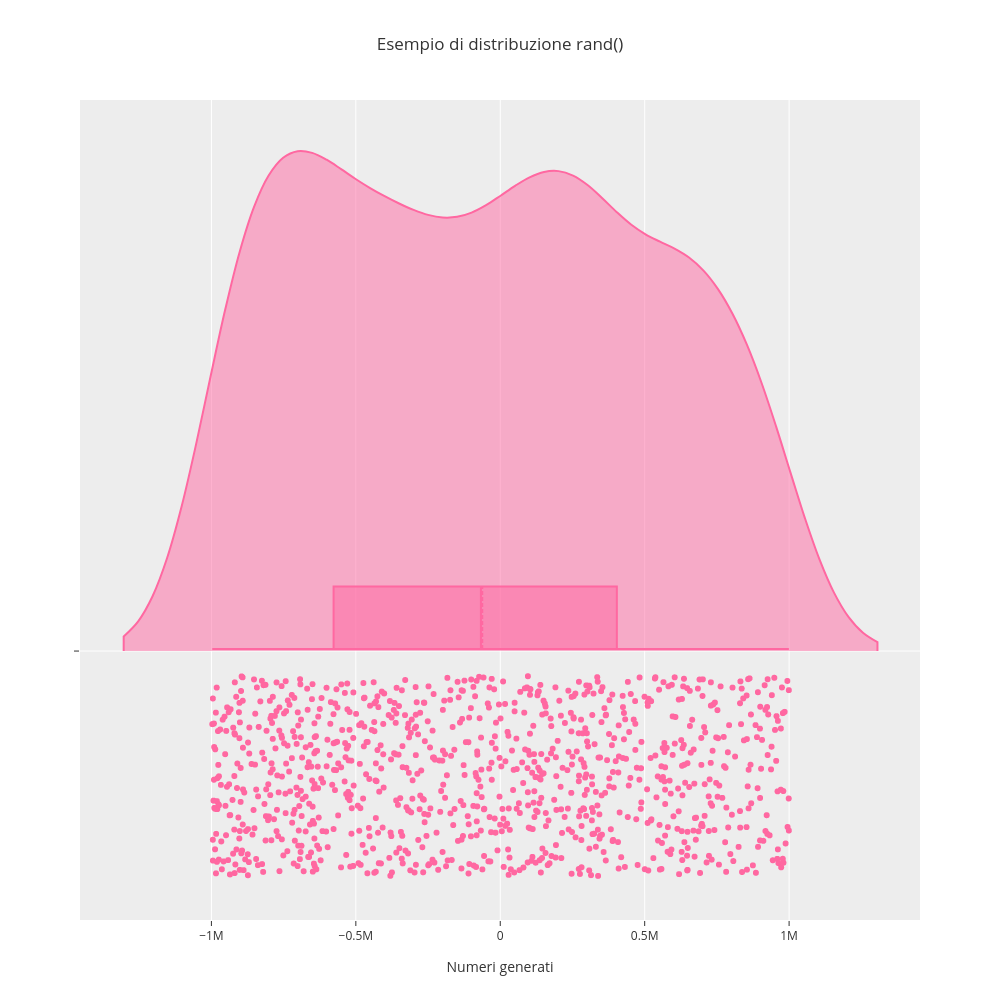
\includegraphics[width=0.68\textwidth]{rand.png}
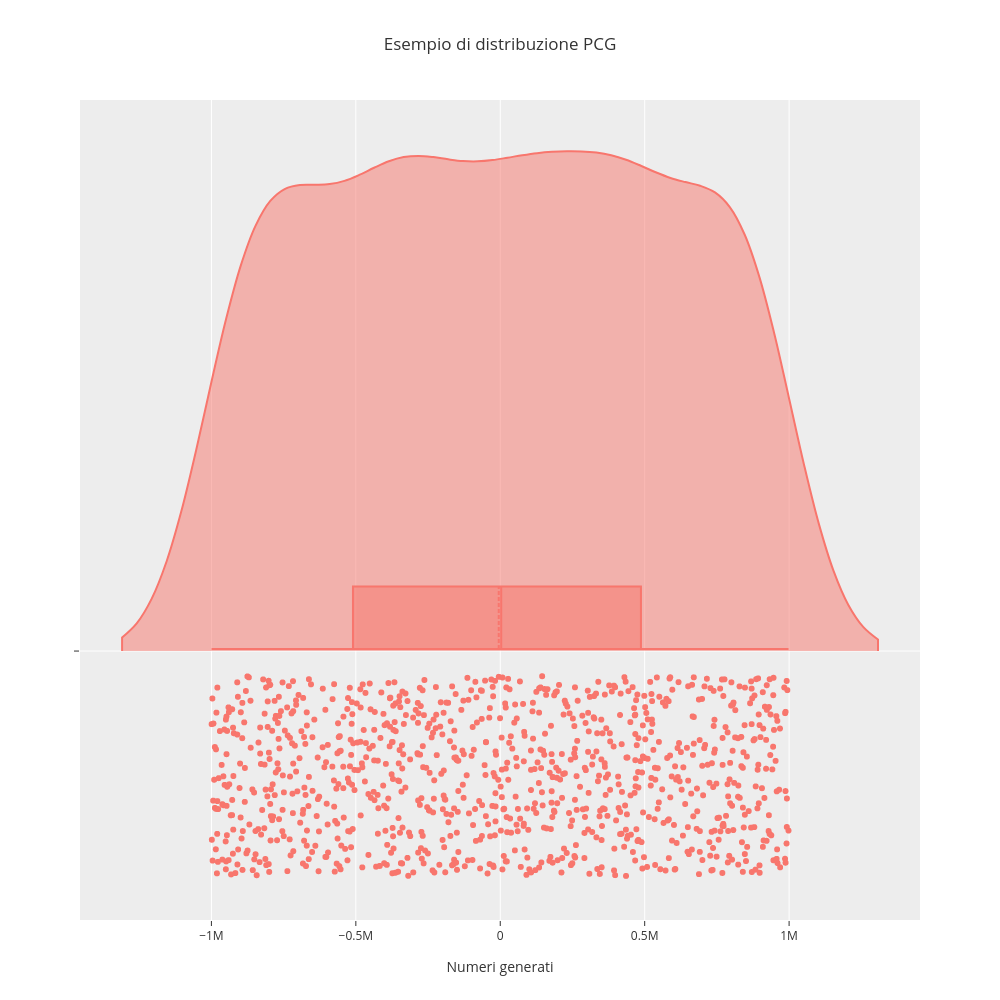
\includegraphics[width=0.68\textwidth]{pcg.png}
\end{center}

\newpage

\subsection{Raccolta dei dati}
I dati vengono raccolti a parità di input e chiave tra gli algoritmi e per lo stopwatch monotono vengono nuovamente impiegati i metodi utilizzati per la stima della risoluzione del clock di sistema.
\newline
\newline
Ad ogni iterazione (il cui numero dipende dal parametro \mintinline{C}{m}) viene popolato un vettore di input (di lunghezza campione che rimane fissa per le \mintinline{C}{m} iterazioni) e viene generata una chiave \mintinline{C}{k}.
\newline
Lo stopwatch viene settato e, sempre come da indicazioni, si entra in un ciclo do-while dove si permane finché l'intervallo di tempo calcolato (aggiornato senza interrompere il ciclo) è minore del tempo minimo rilevabile \mintinline{C}{t_min}.
\newline
\newline
Ad ogni iterazione del ciclo do-while un contatore \mintinline{C}{c} viene incrementato in modo da poter poi ricavare il tempo "medio ammortizzato" dividendo l'intervallo di tempo complessivo passato nel ciclo per il numero di iterazioni.
\newline
La stessa procedura si ripete per ogni algoritmo di selezione, ovviamente contatori e orologio vengono resettati.
\newline
\newline
All'uscita di ognuno dei 3 cicli do-while cronometrati avviene la stampa su file .csv di un record che contiene: campione (dimensione dell'input), chiave e \textit{tempo cronometrato / iterazioni} per ogni algoritmo.
\newline
Solo dopo \mintinline{C}{m} iterazioni si passa al campione successivo.
\newline
\newline
Successivamente è stata implementata una versione multi-thread del programma per la stima dei tempi che, seppur molto semplice, ci ha permesso di dimezzare i tempi necessari alla raccolta dei dati e fornito ulteriori garanzie per quanto riguarda l'indipendenza delle procedure al costo di un consumo di memoria maggiore.
\newline
\newline
Per quanto riguarda i parametri scelti ci si è immediatamente accorti che non era necessario un numero così elevato di campioni (parametro \mintinline{C}{n} $= 500$ nei primi grafici) e che un valore simile comportava problemi di leggibilità.
\newline
Si è deciso quindi per i grafici comparativi tra gli algoritmi di selezione di testare 100 campioni.
\newline
\newline
Sono state fatte diverse sperimentazioni sul numero di iterazioni per campione (parametro \mintinline{C}{m}) al fine di filtrare alcune anomalie causate dall'ambiente di esecuzione. Rilevato che anche un valore elevato non portava benefici per i campioni piccoli si è trovato in 10 un compromesso che permette di produrre risultati affidabili.

\subsection{Analisi dei dati}
L'analisi dei dati si svolge tramite uno script R, per separare la raccolta dei dati dalla loro elaborazione.
\newline
\newline
Uno script bash rielabora l'output del programma per la stima dei tempi per portarlo in formato tidy$^4$:
\newline
\mintinline{BASH}{<tempo>,<campione>,<algoritmo>}.
\newline
\newline
Successivamente richiama su di esso uno script R.
\newline
\newline
Lo script R calcola media e deviazione standard di ogni campione e produce poi due grafici.
\newline
Il primo grafico è in scala lineare, il secondo è in scala doppiamente logaritmica.
\newline
Ogni grafico presenta una curva per algoritmo.
\newline
\newline
La posizione di ogni punto è data dal campione e dalla \textbf{media} dei tempi ammortizzati per quel campione.
\newline
I punti sono collegati da una semplice retta.
\newline
\newline
Solo nel grafico in scala lineare ogni punto è attraversato da una error bar (priva di segmento orizzontale per motivi di leggibilità) tramite la quale viene rappresentata la \textbf{deviazione standard}.
\newline
\newline
Una sottile curva interpola i punti tramite funzione \mintinline{R}{loess}.
\newline
Abbiamo usato questo strumento in fase di sviluppo per capire l'andamento dei tempi, può essere del tutto ignorata.
\newline
\newline
\newline
\newline
\newline
\newline
\href{https://vita.had.co.nz/papers/tidy-data.html}{4. Tidy data}

\newpage

\subsection{Esecuzione}
Il programma per la stima dei tempi viene eseguito tramite uno script bash.
\newline
Oltre ai parametri trattati in precedenza è possibile scegliere se si vuole eseguire una stima simultanea su tutti gli algoritmi (che quindi verranno eseguiti su medesimo input con medesima chiave) o se si vuole profilare uno solo di essi oppure tutti ma distintamente.
\newline
\newline
Lo script chiama la compilazione dei sorgenti, l'esecuzione del programma e provvede poi a concatenare tutti i record e lanciare lo script R che realizza i grafici comparativi.
\newline
\newline
Viste le scelte implementative fatte, particolare cura è stata dedicata alla gestione della memoria.
\newline
\newline
L'implementazione dinamica di Heap Select rende necessario l'utilizzo del metodo \mintinline{C}{free()} anche con input di dimensione modesta se le iterazioni sono numerose.
\newline
\newline
Il programma per la raccolta dei tempi invece è caratterizzato da cicli innestati ed è stato quindi necessario prestare attenzione allo scope delle variabili definite per non superare il limite di memoria per lo stack che nell'ambiente Linux utilizzato era fissato ad un valore standard di circa 40MB.
\newline
L'array di input, seppur per sua natura una struttura dati statica viene ad esempio instanziato con \mintinline{C}{malloc()} in modo tale da occupare la heap invece che lo stack e poter essere liberato quando opportuno.
\newline
\newline
L'esecuzione multi-thread non è veramente parallela in quanto i processi devono aspettarsi prima che avvenga la rigenerazione di input e chiave. Con questi 3 algoritmi è stato normale sfruttare circa 2 thread per tutta l'esecuzione dato che Heap Select e Median of Medians Select hanno tempi di esecuzione abbastanza simili.
\newline
\newline
Non sono stati usati i parametri di ottimizzazione del compilatore GCC in fase di stima dei tempi in quanto si è ritenuto ciò avere poco senso nel contesto dello studio degli algoritmi, si sono però sfruttati per testare la stabilità del profiler e far emergere alcuni errori di programmazione.
\newline
\newline
Soprattutto su campioni piccoli si sono rilevate anomalie che ci sentiamo di ricondurre a scheduling, interrupt o meccanismi simili e che solo in parte siamo riusciti a mitigare.
\newline
Nei grafici saranno facilmente riconoscibili in quanto interessano contemporaneamente tutte le curve.
\newline
\newline
Il fenomeno si manifesta con maggiore intensità se il computer è in uso durante l'esecuzione del programma per la stima dei tempi. Non abbiamo individuato pattern ricorrenti.
\newline
\newline
É stato dedicato molto tempo a cercare di evitare le anomalie di cui sopra ma come detto in precedenza anche aumentare il numero di iterazioni non ha portato benefici per i campioni più piccoli. Le iterazioni venendo eseguite una di seguito all'altra, se i campioni sono piccoli avvengono in tempo breve e finiscono per essere tutte interessate.

\section{Aspettative teoriche}
Si riassumono ora le aspettative teoriche maturate in base a quanto: studiato nel corso, indicato in fase di descrizione del progetto e ricavato dalla fonti bibliografiche consultate.
\newline
\newline
\textbf{Quick Select}
\newline
Ci si aspetta di stimare complessità $\Theta(n)$ e che però rimanga traccia della complessità quadratica nel caso pessimo.
\newline
\newline
\textbf{Heap Select}
\newline
Ci si aspetta di stimare complessità $O(n + k log k)$ e di rilevare buone prestazioni per $k$ piccoli.
\newline
\newline
\textbf{Median of Medians Select}
\newline
Ci si aspetta di stimare complessità $\Theta(n)$, si ritiene che i passaggi necessari alla selezione del pivot possano comportare tempi in senso assoluto superiori rispetto a Quick Select che dovrebbe essere il più veloce del lotto.

\newpage

\section{Risultati empirici}
\begin{center}
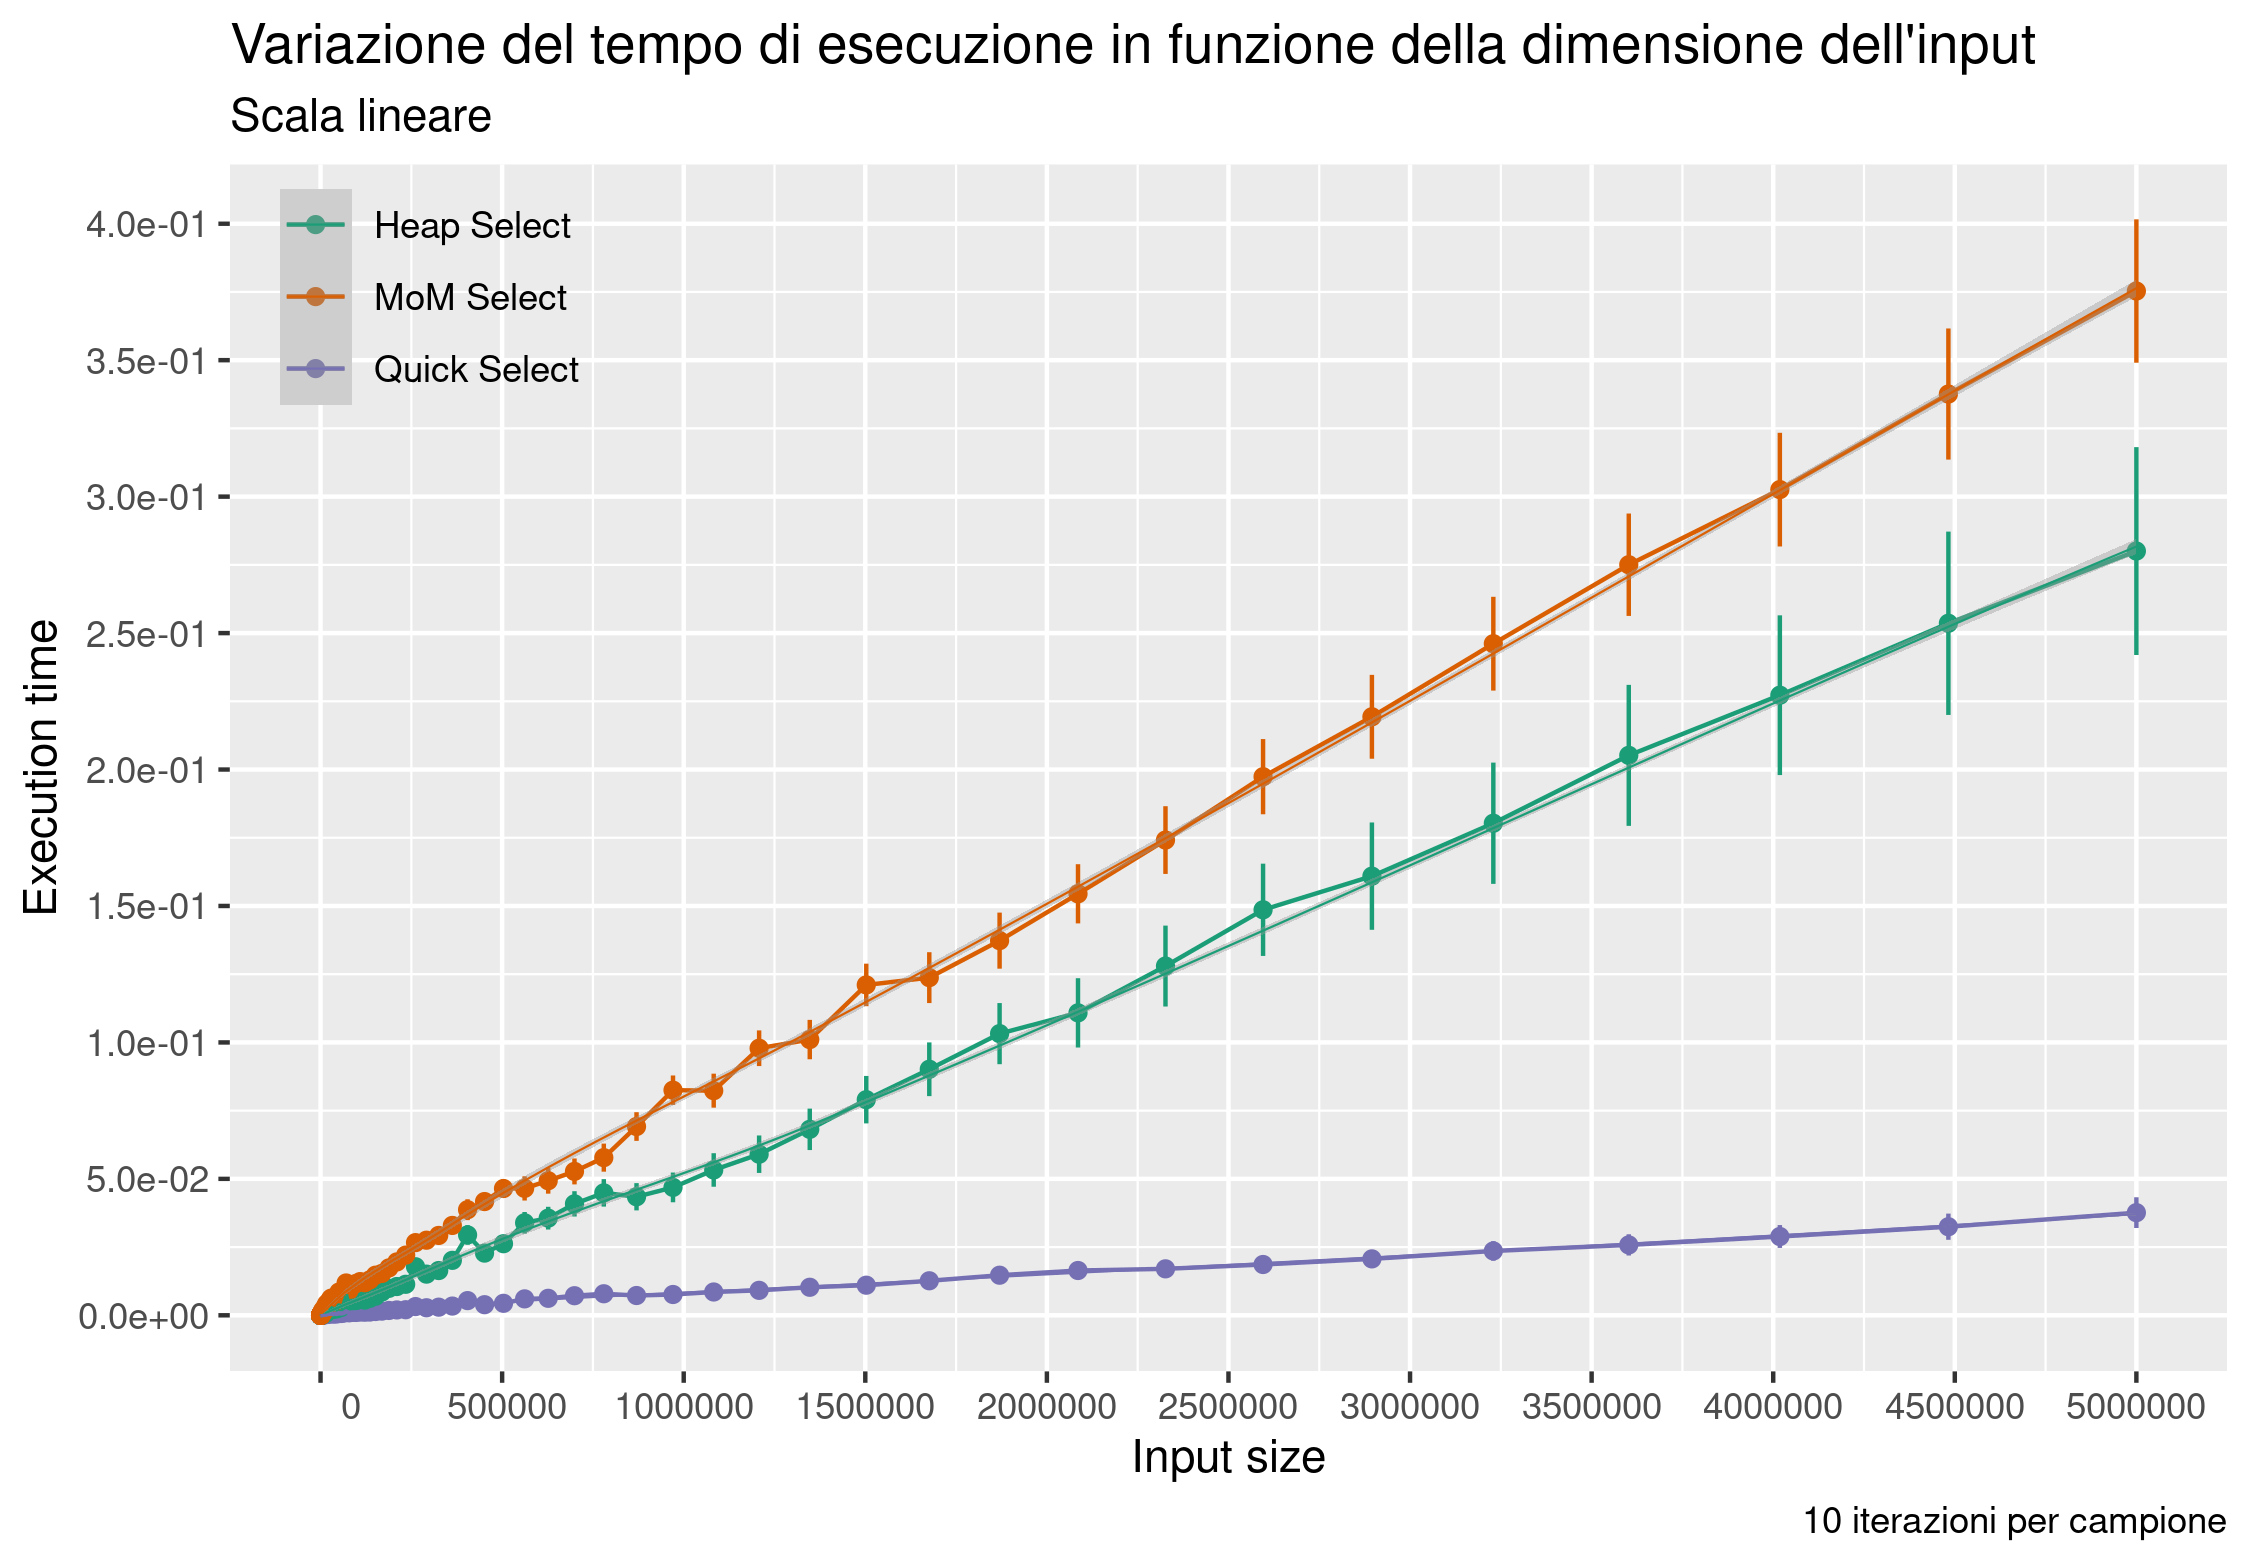
\includegraphics[width=\textwidth]{p_lin.png}
\end{center}
Le aspettative relative alla complessità asintotica degli algoritmi paiono rispettate.
\newline
\newline
Heap Select mostra la maggiore deviazione standard, il che ci pare corretto in quanto è l'unico algoritmo la cui complessità asintotica dipende anche dalla chiave, che ricordiamo, varia a ogni iterazione.
\newline
\newline
Purtroppo per motivi di scala non si riesce a valutare la deviazione standard di Quick Select, guardando però i record e basandoci anche su quanto visto nel primo capitolo possiamo concludere che complessivamente l'algoritmo si colloca tra Median of Medians Select (il migliore da questo punto di vista) e Heap Select.
\newline
Anche questo ci pare corretto in quanto Median of Medians Select dedica dei passaggi alla scelta del pivot ottimale mentre Quick Select si espone alla possibile scelta di un cattivo pivot.
\newline
\newline
Sorprendono la prestazioni di Quick Select anche se già per quanto visto in precedenza si era dimostrato molto veloce e con una buona complessità nel caso medio. Non ci si aspettava però un tale distacco.
\newline
\newline
Allo stesso modo è stato inatteso rilevare prestazioni così simili tra Median of Medians Select e Heap Select. Ci saremmo poi aspettati che le operazioni necessarie alla costruzione e gestione della heap avrebbero avuto un peso maggiore rispetto alle operazioni che Median Select svolge su un semplice vettore, così non è stato.
\newline
\newline
Un'ulteriore conclusione che ci sentiamo di trarre è relativa all'input, evidentemente gli accorgimenti impiegati ci hanno permesso di generare una distribuzione piuttosto uniforme.

\newpage
\begin{center}
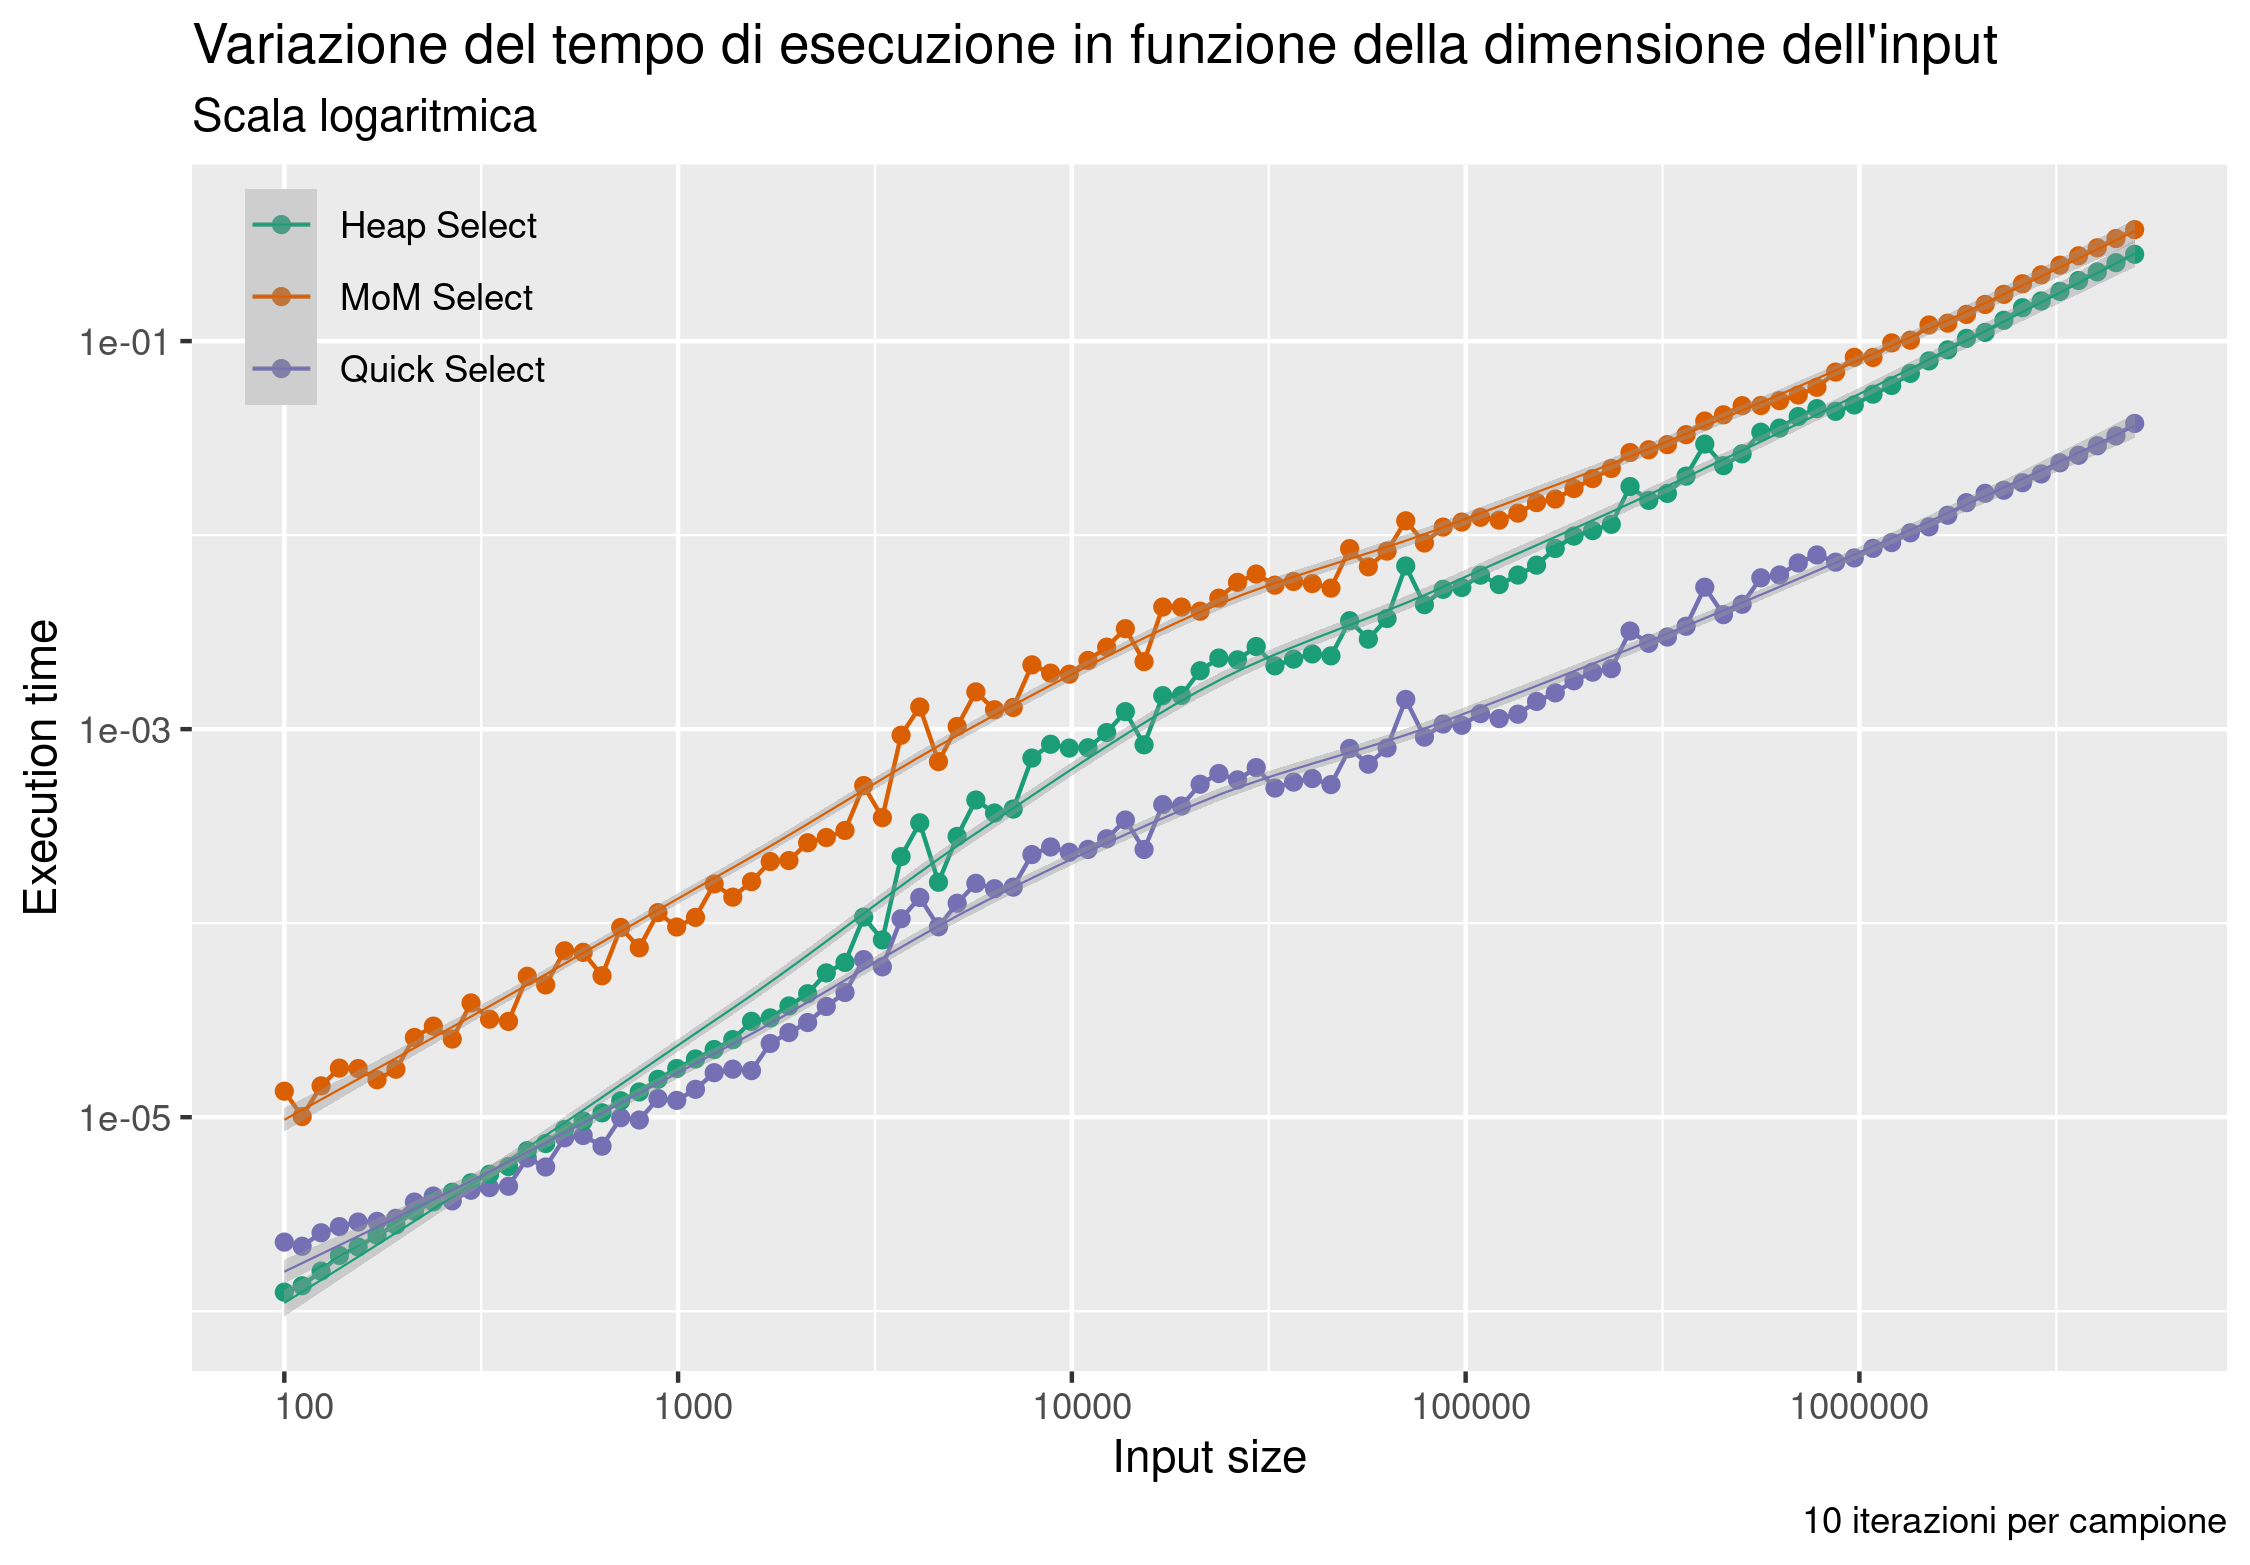
\includegraphics[width=\textwidth]{p_log.png}
\end{center}
La scala doppiamente logaritmica ci permette di valutare una questione rimasta in sospeso, l'aspettativa relativa a Heap Select per k piccoli: effettivamente Heap Select si dimostra competitivo con Quick Select sui campioni di dimensione più contenuta, nei quali è ovviamente più probabile incontrare k piccolo vista la correlazione tra range della chiave e dimensione dell'input.
\newline
\newline
Sempre grazie a questo grafico, facendo tara delle anomalie che purtroppo interessano la zona centrale, si può notare che Heap Select ha una crescita sensibilmente più sostenuta rispetto agli altri due algoritmi.
\newline
Questo a conferma delle aspettative teoriche, anche se sfortunatamente non emerge con chiarezza dal grafico lineare.
\newline
\newline
Prima di concludere si vuole fare qualche valutazione empirica sulla complessità spaziale:
\newline
abbiamo rilevato il comportamento migliore da parte di Median of Medians Select, seguito da Quick Select che probabilmente è penalizzato dal un numero maggiore di chiamate ricorsive eseguite.
\newline
Il quantitativo di memoria allocato da Heap Select è ulteriormente superiore, per lo meno con questa nostra implementazione.

\newpage

\section{Conclusioni}
L'implementazione degli algoritmi discussi e l'analisi presentata ci hanno permesso di consolidare e applicare le conoscenze teoriche acquisite durante il corso e di trovare sostanziale conferma delle aspettative maturate.
\newline
\newline
Sono inoltre emersi dettagli del comportamento degli algoritmi che non avremmo avuto modo di conoscere senza un'analisi empirica quali ad esempio l'uso della memoria, gli effetti di certe scelte implementative e l'ordine di grandezza dei tempi di esecuzione.
\newline
\newline
Alla luce di quanto visto e senza considerare quindi eventuali algoritmi più avanzati, si ritiene che un'implementazione ottimizzata di Quick Select possa essere la scelta ottimale per risolvere un problema generale di selezione. Per applicazioni pratiche bisognerà invece valutare caso per caso quali strutture dati e algoritmi implementare.

\vspace{15cm}
\section*{Contatti}
\href{mailto:antonutti.marco001@spes.uniud.it}{antonutti.marco001@spes.uniud.it}
\newline
\newline
\href{mailto:pipan.martin@spes.uniud.it}{pipan.martin@spes.uniud.it}
\newline
\newline
\href{mailto:candolo.vittoriogiorgio@spes.uniud.it}{candolo.vittoriogiorgio@spes.uniud.it}

\end{document}